\scanpage{7}

formellement sur le diagramme des deux suites transposées l'une de l'autre
\diagram{\begin{tikzcd}[ampersand replacement=\&]
A\arrow[r,"F"]\&A^{(p)}\arrow[r,"V"]\&\unsure{V|A}\\[1.8em]
B\&B^{(p)}\arrow[l,"V"']\&B\arrow[l,"F"']
\end{tikzcd}}
On trouve ainsi la suite exacte
\diagram{\begin{tikzcd}[ampersand replacement=\&]
0\arrow[r,no head]\&\operatorname{Gr}(\uline{t}_A)\arrow[r,no head]\&p^A\arrow[r]\&D(\operatorname{Gr}(\uline{t}_B))\arrow[r]\&0
\end{tikzcd}}
extension canonique de $\unsure{D}(F_{\deleted{\unsure{A}}}^{B})$ par $F^A$.

Noter d'ailleurs que $S_A$ est une extension de $p$-alg. de Lie abéliennes\inserted{\figure{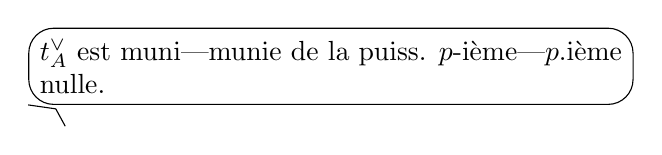
\begin{tikzpicture}
\node[draw,rounded corners=9pt,align=left,inner sep=4pt] (a) {$t_A^\vee$ est \unsure{muni|munie} de la puiss. \unsure{$p$-ième|$p$.ième}\\nulle.};
\draw (a.south west)--++(.35,-.05)--++(.12,-.22);
\end{tikzpicture}}}, et correspond donc en fait à une extension de groupes radiciels. Cette extension peut-elle se déduire de la connaissance de $p^A$ ??

\mspage{6}
